\documentclass[tikz, border=0pt]{standalone}
\usetikzlibrary{patterns,angles,quotes}

\begin{document}
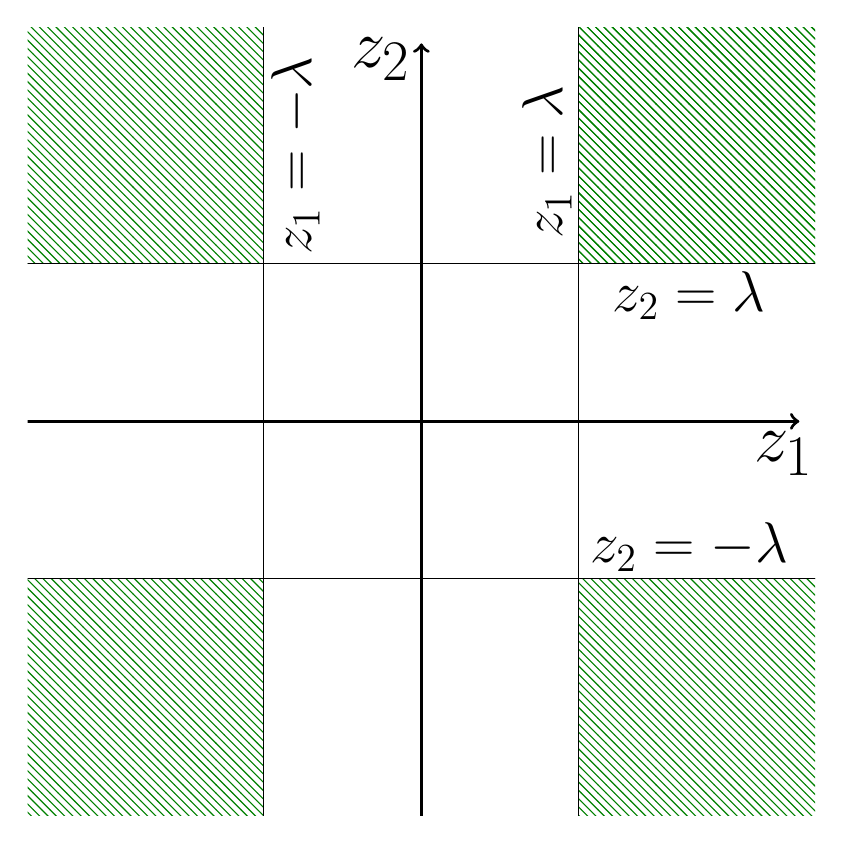
\begin{tikzpicture}
    % Draw and hatch a rectangle
    % \draw[fill, pattern=north west lines, pattern color=blue] (0,0) rectangle (4,2);

    % % Draw and hatch a custom polygon
    % \draw[fill, pattern=crosshatch dots, pattern color=red] (5,0) -- (7,3) -- (9,1) -- cycle;

    % % Draw and hatch a circle
    % \draw[fill, pattern=grid, pattern color=green!50!black] (12,1) circle (1.5);

    % \coordinate (A) at (2,0);
    % \coordinate (B) at (0,0);
    % \coordinate (C) at (1,1);

    % \draw (A) -- (B) -- (C); % Draw the lines forming the angle

    % \pic [draw,fill,  pattern=grid, pattern color=green!50!black] {angle = A--B--C}; % Draw and label the angle arc

    % \coordinate (D) at (3,0);
    % \coordinate (E) at (0,0);
    % \coordinate (F) at (1,2);
    
    % \draw (D) -- (E) -- (F);
    
    % \pic[draw, angle radius=1cm, "$\Vert$"] {angle = D--E--F}; % Use `$\Vert$` for double hash

   
    % Define the clipping region for the first quadrant
    \clip (-5,-5) rectangle (5,5);

    % Fill the region below y = 1/x
    \path[pattern=north west lines, pattern color=green!50!black] 
        (2,2) -- (5.2,2) -- (5.2,5.2) -- (2,5.2) -- cycle;

            \path[pattern=north west lines, pattern color=green!50!black] 
        (2,2) -- (5.2,2) -- (5.2,5.2) -- (2,5.2) -- cycle;

            \path[pattern=north west lines, pattern color=green!50!black] 
        (-2,2) -- (-5.2,2) -- (-5.2,5.2) -- (-2,5.2) -- cycle;

            \path[pattern=north west lines, pattern color=green!50!black] 
        (2,-2) -- (5.2,-2) -- (5.2,-5.2) -- (2,-5.2) -- cycle;
        
          \path[pattern=north west lines, pattern color=green!50!black] 
        (-2,-2) -- (-5.2,-2) -- (-5.2,-5.2) -- (-2,-5.2) -- cycle;
    % Draw the main curve and axes
    % \draw[thick, blue, domain=1:5] plot[samples=100] (\x, {1/\x});
    \draw[->,very thick] (0-5.2,0) -- (4.8,0) node[below] at (4.6,0) {\Huge $z_1$};
    \draw[->,very thick] (0,-5.2) -- (0,4.8) node[left] at (0,4.6) {\Huge $z_2$};

    \draw (2,-5.2) -- (2,5.2) node[right, rotate=90] at (1.6,2.2) {\huge $z_1=\lambda$};

    \draw (-2,-5.2) -- (-2,5.2) node[right, rotate=90] at (-1.6,2) {\huge $z_1=-\lambda$};

    \draw (-5.2,2) -- (5.2,2) node[ rotate=0] at (3.4,1.6) {\huge $z_2=\lambda$};


    
    \draw (-5.2,-2) -- (5.2,-2) node[ rotate=0] at (3.4,-1.6) {\huge $z_2=-\lambda$};
    % Draw a point to show the boundary starts at x=1
    % \filldraw[black] (1,1) circle (2pt);
    % \node[below] at (1,0) {1};
    % \node[left] at (0,1) {1};
    
    % Add the label
    % \node[above, right, blue] at (3,0.5) {$y = 1/x$};


\end{tikzpicture}
\end{document}